\subsection{Библиотека Хьюза}

Библиотека Джона Хьюза\cite{hughes} считается первой комбинаторной принтер-библиотекой. Она основана на алгоритме, предложенном Дереком Оппеном \cite{oppen}, и по сути является его реализацией в функциональном стиле на языке Haskell\footnote{http://haskell.org}. Также библиотека Хьюза, расширенная Саймоном Пейтоном Джонсом \cite{peytonJones}, является стандартной принтер-библиотекой для языка Haskell.

% рассказать об оптимальном

В данной библиотеке ключевым типом является “\lstinline[language=Haskell]{Doc}”. Он представляет документ, который потом может быть переведен в строковое представление.
Основные комбинаторы для составления документа:
% \inputminted{haskell}{Podkopaev/codes/hughesBasicOperators.hs}
\lstinputlisting[language=Haskell]{Podkopaev/codes/hughesBasicOperators.hs}

Так, с помощью функции “\lstinline[language=Haskell]{text}” по строке получается документ, оператор “\textbf{<>}” соединяет два документа горизонтально (см. рисунок~\ref{fig:hughesHorComp}), а оператор “\textbf{\$\$}” соединяет документы вертикально (см. рисунок~\ref{fig:hughesVertComp}).

\begin{figure}[ht]
	\begin{subfigure}[b]{0.45\linewidth}
		\centering
		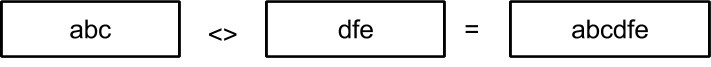
\includegraphics[width=\textwidth]{hughesHorComp}
		\caption{Комбинатор “\textbf{<>}”}
		\label{fig:hughesHorComp}
	\end{subfigure}
	\hspace{0.5cm}
	\begin{subfigure}[b]{0.45\linewidth}
		\centering
		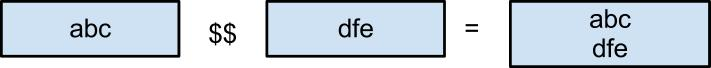
\includegraphics[width=\textwidth]{hughesVertComp}
		\caption{Комбинатор “\textbf{\$\$}”}
		\label{fig:hughesVertComp}
	\end{subfigure}

	\caption{Пример работы комбинаторов}
\end{figure}

Функция “\lstinline[language=Haskell]{nest}” добавляет к каждой строке документа заданное число ведущих пробелов. Функция “\lstinline[language=Haskell]{sep}” является ключевым комбинатором, который в этой библиотеке позволяет задавать плавающую раскладку документа. Она принимает как параметр список документов, а на выходе получается документ, который представляет из себя либо вертикальную склейку элементов списка, либо горизонтальную склейку (в этом случае если к документу из списка применялась функция “\lstinline[language=Haskell]{nest}”, то к этому документу не добавляются ведущие пробелы, то есть применение “\lstinline[language=Haskell]{nest}” попросту игнорируется), причем между документами вставляется пробельный символ. Вариант раскладки выбирается функцией “\lstinline[language=Haskell]{pretty}”:

% \inputminted{haskell}{Podkopaev/codes/hughesPretty.hs}
\lstinputlisting[language=Haskell]{Podkopaev/codes/hughesPretty.hs}

Кроме самого документа, функция “\lstinline[language=Haskell]{pretty}” также принимает два числа: максимальную длину и максимальную наполненность строки. Здесь наполненность строки значит длину текста без ведущих пробельных символов. В ходе работы этой функции и происходит выбор раскладки документа, полученного с помощью комбинатора “\lstinline[language=Haskell]{sep}”. Если горизонтальная раскладка удовлетворяет ограничениям на ширину строки, то она и выбирается. Иначе выбирается вертикальная раскладка.


% Возможно, стоит сделать после обзора всех библиотек

Рассмотрим пример описания принтера с помощью библиотеки Хьюза. Для этого используем учебный язык L. Часть принтера для языка L, отвечающая за представление операторов, показана на рисунке~\ref{fig:lHughesPrinter}.
В примере используется не описанный выше комбинатор “\lstinline[language=Haskell]{<+>}”, который определяется следующим образом:

\lstinputlisting[language=Haskell]{Podkopaev/codes/hughesAddComb.hs}

\begin{figure}[h!]
	% \inputminted{haskell}{Podkopaev/codes/lHughesPrinter.hs}
	\lstinputlisting[language=Haskell]{Podkopaev/codes/lHughesPrinter.hs}
	\caption{Принтер, написанный с помощью библиотеки Хьюза}
	\label{fig:lHughesPrinter}
\end{figure}

В данном случае принтер получился несложным, но абсолютно не наглядным. Поскольку в библиотеке нет механизмов, позволяющих явно варьировать раскладку документа в зависимости от раскладки его поддокументов, невозможно выразить пример с рисунка~\ref{fig:lGoodWriteEx}.
То есть, в случае многострочного выражения в операторе “\lstinline[language=llang]{write}”, напечатать закрывающую скобку на уровне самого оператора.

\begin{figure}[h!]
	% \inputminted{pascal}{Podkopaev/codes/lGoodWriteEx.l}
	\lstinputlisting[language=llang]{Podkopaev/codes/lGoodWriteEx.l}
	\caption{Желательный пример печати конструкции “\lstinline[language=llang]{write}”}
	\label{fig:lGoodWriteEx}
\end{figure}

С помощью реализации принтера с рисунка~\ref{fig:lHughesPrinter}, в данном случае для оператора “\lstinline[language=llang]{write}” получится немного не то (см. рисунок~\ref{fig:lCurWriteEx}).
\begin{figure}[h!]
	% \inputminted{pascal}{Podkopaev/codes/lCurWriteEx.l}
	\lstinputlisting[language=llang]{Podkopaev/codes/lCurWriteEx.l}
	\caption{Результат для изначального принтера конструкции “\lstinline[language=llang]{write}”}
	\label{fig:lCurWriteEx}
\end{figure}

Если попробовать поменять функцию “\lstinline[language=Haskell]{docFromOperation}” для конструкции “\lstinline[language=llang]{write}” (см. рис. \ref{fig:lHughesWriteChange}),
то для многострочного выражения все получится правильно, но в случае однострочного --- появится лишний пробел перед закрывающей скобкой (см. рис. \ref{fig:lBadWriteEx})).

\begin{figure}[h!]
	% \inputminted{haskell}{Podkopaev/codes/lHughesWriteChange.hs}
	\lstinputlisting[language=Haskell]{Podkopaev/codes/lHughesWriteChange.hs}
	\caption{Измененный принтер конструкции “\lstinline[language=llang]{write}”}
	\label{fig:lHughesWriteChange}
\end{figure}

\begin{figure}[h!]
	% \inputminted{pascal}{Podkopaev/codes/lBadWriteEx.l}
	\lstinputlisting[language=llang]{Podkopaev/codes/lBadWriteEx.l}
	\caption{Результат для измененого принтера конструкции “\lstinline[language=llang]{write}”}
	\label{fig:lBadWriteEx}
\end{figure}